\documentclass[]{article}

% Use utf-8 encoding for foreign characters
%\usepackage[latin1]{inputenc}


% Setup for fullpage use
\usepackage{fullpage}
% Uncomment some of the following if you use the features
%
% Running Headers and footers
%\usepackage{fancyhdr}

% Multipart figures ´¡009753º
% More symbols
%\usepackage{amsmath}\emph{}
%\usepackage{amssymb}
%\usepackage{latexsym}

% Surround parts of graphics with box
\usepackage{boxedminipage}

% Package for including code in the document
\usepackage{listings}

% Package for subfigure
\usepackage{graphicx}


% If you want to generate a toc for each chapter (use with book)
\usepackage{minitoc}

% This is now the recommended way for checking for PDFLaTeX:
\usepackage{ifpdf}
%\newif\ifpdf
%\ifx\pdfoutput\undefined
%\pdffalse % we are not running PDFLaTeX
%\else
%\pdfoutput=1 % we are running PDFLaTeX
%\pdftrue
%\  XCM CNXKJBWQGFUHREPUYT485¨94-32¨1fi
\usepackage[all,light]{draftcopy}
%\draftcopyName{PROBABILIDAD II}{5}


\usepackage{amsmath}
\usepackage{amsfonts}
\usepackage{bm}
\usepackage{layout}
\usepackage{fancyhdr}
\usepackage{subcaption}
\pagestyle{fancy}
%\fancyhf{}
\newlength\FHoffset
\setlength\FHoffset{0.1cm}
%\addtolength\headwidth{2\FHoffset}
\fancyheadoffset{\FHoffset}
%\ifpdf
%\usepackage[pdftex]{graphicx}
%\else
%\usepackage{graphicx}
%\fi
\usepackage[top=2cm,bottom=2cm,left = 1cm, right = 1cm,headsep=1.5cm]{geometry}
\usepackage{hyperref}
\newcommand{\R}{\mbox{$I\!\!R$}}
\usepackage{cleveref}

\begin{document}

\lhead{\textsf{UCSC - Fall 2016} \\{AMS 374}}
\chead{\Large{General Linear Model}}
\rhead{\textsf{Student:} \\{Rui Meng}}
\renewcommand{\headrulewidth}{0.4pt}
\renewcommand{\footrulewidth}{0.4pt}


\begin{center}
\section*{\underline{Homework 4}}
\end{center}

\begin{enumerate}  \Large{
		\item[Ex1] The table below reports results from a developmental toxicity study involving ordinal categorical outcomes. This study administered diethylene glycol dimethyl ether (an industrial solvent used in the manufacture of protective coatings) to pregnant mice. Each mouse was exposed to one of five concentration levels fro ten days early in the pregnancy (with concentration 0 corresponding to controls). Two days later, the uterine contents of the pregnant mice were examined for defects. One of three (ordered) outcomes ("Dead", "Malformation", "Normal") was recorded for each fetus.
		\begin{table}[ht!]
			\centering
			\begin{tabular}{c|c c c|c}
				\hline
				Concentration    &          & Response       &                & Total number  \\
				(mg/kg per day) & Dead & Malformation & Normal   & of subjects      \\
				($x_i$)               & ($y_{i1}$) & ($y_{i2}$) & ($y_{i3}$) & ($m_i$)           \\
				\hline
				0                       & 15      & 1                    & 281         & 297                 \\
				62.5                  & 17      & 0                    & 225         & 242                 \\
				125                   & 22      & 7                    & 283         & 312                 \\
				250                   & 38      & 59                  & 202         & 299                 \\
				500                   & 144     & 132               & 9             & 285                 \\
				\hline
			\end{tabular}
		\end{table}
		Build a multinomial regression model for these data using continuation-ratio logits for the response probabilities $\pi_j(x), j = 1,2,3$, as a function of concentration level, $x$, Specifically, consider the following model 
		$$L_1^{(cr)} = \log(\frac{\pi_1}{\pi_2+\pi_3}) = \alpha_1 + \beta_1 x; L_2^{(cr)} = \log(\frac{\pi_2}{\pi_3}) = \alpha_2 + \beta_2 x$$
		for the multinomial response probabilities $\pi_j \equiv \pi_j(x), j = 1,2,3$.
		\begin{itemize}
			\item[(a)] Show that the model, involving the multinomial likelihood for the data $= \{(y_{i1}, y_{i2}, y_{i3}, x_i) : i = 1,\ldots,5\}$, can be fitted by fitting separately two Binomial GLMs. Provide details for your argument, including the specific form of the Binomial GLMs.
			\item[(b)] Use the result from part (a) to obtain the MLE estimates and corresponding standard errors for parameters $(\alpha_1, \alpha_2, \beta_1, \beta_2)$. Plot the estimated response curves $\hat{\pi}_j(x)$, for $j = 1,2,3$, and discuss the results
			\item[(c)] Develop and implement a Bayesian version of the model above. Discuss your prior choice, and provide details for the posterior simulation method. Provide point and interval estimates for the response curves $\pi_j(x)$ for $j = 1,2,3$.
		\end{itemize}
		
		\item[Sol 1]
		\begin{itemize}
			\item[(a)]
			The multinomial likelihood can be expressed as 
			\begin{eqnarray}
			L(\pi_1,\pi_2,\pi_3| \bm m, \bm y)  & = &  \prod_{i = 1}^{5}\frac{m_i!}{\prod_{j = 1}^{3}y_{ij}!}\pi_1^{y_{i1}} \pi_2^{y_{i2}} (1-\pi_1-\pi_2)^{y_{i3}}\\
			& = & \prod_{i = 1}^{5} \frac{m_i!}{y_{i1}!(m_i - y_{i1})!}\pi_{1}^{y_{i1}}(1-\pi_{1})^{m_i - y_{i1}}\\
			& &\frac{(m_i-y_{i1})!}{y_{i2}! y_{i3}!}(\frac{\pi_{2}}{1-\pi_{1}})^{y_{i2}} (\frac{1-\pi_1-\pi_2}{1-\pi_1})^{y_{i3}}\,,
			\end{eqnarray}
			which implies that $Mult(\bm y| \bm m, \bm \pi) = Bin(y_1| m, \pi_1) \times Bin(y_2| m-y_1, \frac{\pi_2}{1-\pi_1})$. So the multinomial distribution of $\bm y$ can be regards as a joint distribution of two independent Binomial distributions. Then fitting the multinomial distribution is equal to fitting two independent binomial distributions.
			\item[(b)]
			The MLE estimates and corresponding standard errors for parameters ($\alpha_1$, $\alpha_2$, $\beta_1$, $\beta_2$) are in Table~\ref{MLE}.
			\begin{table}[ht!]
				\centering
				\caption{MLE estimate and standard error}
				\begin{tabular}{c|c|c|c|c}
					\hline
					                 &  $\alpha_1$  &  $\alpha_2$  &  $\beta_1$  &  $\beta_2$  \\
					\hline
					 Estimate  &  -3.25  &  -5.70  & 0.01   &   0.02 \\
					 \hline
					 SE           &   0.16   &   0.33    &  0.00  &   0.00 \\
					 \hline
				\end{tabular}
				\label{MLE}
			\end{table}
			The estimated response curves $\hat{\pi}_j(x)$ are plotted in Figure~\ref{ERC}.
			\begin{figure}[ht!]
				\centering
				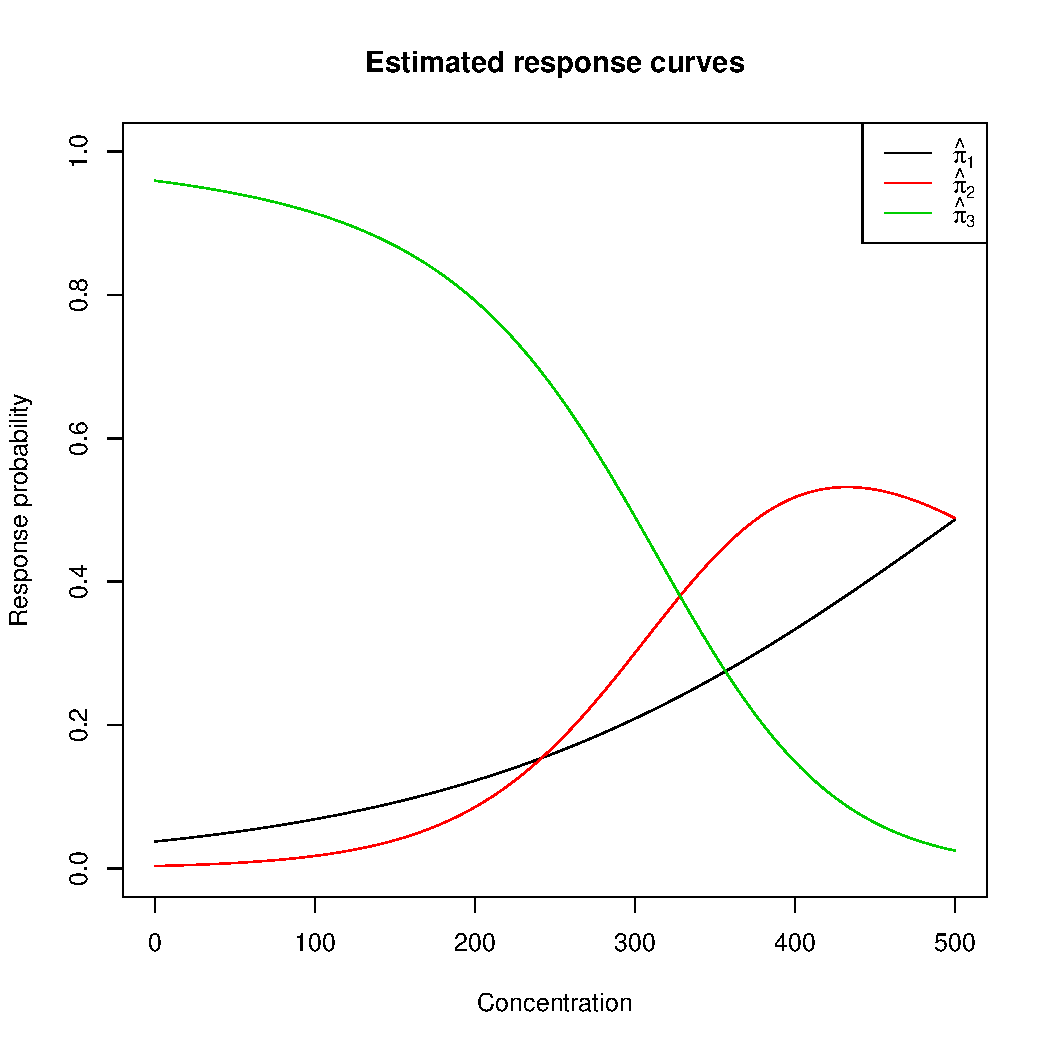
\includegraphics[scale = 0.5]{pic/HW4_1/ERC}
				\caption{Estimated response curves}
				\label{ERC}
			\end{figure}
			As the concentration increases, more and more mice become ill even dead. 
			\item[(c)]
			The posterior distribution of parameters can be expressed as below:
			{\footnotesize
			\begin{eqnarray}
			Pr(\bm \alpha, \bm \beta|\bm x, \bm y, \bm m) & \propto & Pr(\bm \alpha, \bm \beta) f(\bm y|\bm m, \bm x, \bm \alpha, \bm \beta)\\
			& = & Pr(\bm \alpha, \bm \beta) \prod_{i = 1}^{5} \frac{m_i!}{y_{i1}!(m_i - y_{i1})!}(\frac{1}{1+\exp(-(\alpha_1 + \beta_1 x_i))})^{y_{i1}}(\frac{\exp(-(\alpha_1 + \beta_1 x_i))}{1+\exp(-(\alpha_1 + \beta_1 x_i))})^{m_i - y_{i1}}\\
			& &\frac{(m_i-y_{i1})!}{y_{i2}! y_{i3}!}(\frac{1}{1+\exp(-(\alpha_2 + \beta_2 x_i))})^{y_{i2}} (\frac{\exp(-(\alpha_2 + \beta_2 x_i))}{1+\exp(-(\alpha_2 + \beta_2 x_i))})^{y_{i3}}\\
			& \propto & Pr(\bm \alpha, \bm \beta)\prod_{i = 1}^{5} (\frac{1}{1+\exp(-(\alpha_1 + \beta_1 x_i))})^{y_{i1}}(\frac{\exp(-(\alpha_1 + \beta_1 x_i))}{1+\exp(-(\alpha_1 + \beta_1 x_i))})^{m_i - y_{i1}}\\
			& &(\frac{1}{1+\exp(-(\alpha_2 + \beta_2 x_i))})^{y_{i2}} (\frac{\exp(-(\alpha_2 + \beta_2 x_i))}{1+\exp(-(\alpha_2 + \beta_2 x_i))})^{y_{i3}}
			\end{eqnarray}}
			Since there is no information about parameters $\bm \alpha$, $\bm \beta$, we assume they have flat prior. Then using the Adaptive Metropolis Hasting method, we generate the posterior distribution of $\bm \alpha$ and $\bm \beta$ with $5000$ times sampling and reasonable burn-in. Then based on the $\bm\hat{\alpha}$ and $\bm{\hat{\beta}}$, we provide the point and $95\%$ centered interval estimates for the response curves $\pi_j(x)$ for $j = 1,2,3$ in Figure~\ref{BERC}.
			\begin{figure}[ht!]
				\centering
				\includegraphics[scale = 0.5]{"pic/HW4_1/BERC"}
				\caption{The estimated response curves with their $95\%$ centered interval estimates}
				\label{BERC}
			\end{figure}
		\end{itemize}
		
		\item[Ex 2] Consider the "alligator food choice" data example, the full version of which is discussed in Section 7.1 of Agresti (2002), \textit{Categorical Data Analysis}, Second Edition. Here, consider the subset of the data reported in Table 7.16 (page 304) of the above book, This data set involves observations on the primary food choice for $n=63$ alligators caught in Lake George, Florida. The nominal response variable is the primary food type (in volume) found in each alligator's stomach, with three categories: "fish", "invertebrate", and "other". The invertebrates were mainly apple snails, aquatic insects, and crayfish. The "other" category included amphibian, mammal, bird, reptile, and plant material. Also available for each alligator is covariate information on its length (in meters) and gender.
		\begin{itemize}
			\item[(a)] Focus first on length as the single covariate to explain the response probabilities for the "fishes", "invertebrate" and "other" food choice categories. Develop a Bayesian multinomial regression model, using the baseline-category logits formulation with "fish" as the baseline category, to estimate (with point and interval estimates) the response probabilities as a function of length. (Note that in this data example, we have $m_i = 1$, for $i = 1,\ldots,n$.) Discuss your prior choice and approach to MCMC posterior simulation.
			\item[(b)] Extend the model from part (a) to describe the effects of both length and gender on food choice. Based on your proposed model, provide point and interval estimates for the length-dependent response probabilities for male and female alligators.
		\end{itemize}
		
        \item[Sol 2]
        \begin{itemize}
        	\item[(a)]
        	First of all, we summarize the Table 7.16 by unique length and respective number of three categories. Denote lengths as $x$ and number of three categories as $I$, $F$ and $O$ with probability $\pi_1$, $\pi_2$ and $\pi_3$ and total number as $M$. Then having $O$ as a baseline, we can propose the link functions as 
        	$$\log(\frac{\pi_1}{\pi_3}) = \alpha_1 + \beta_1 x$$
        	and 
        	$$\log(\frac{\pi_2}{\pi_3}) = \alpha_2 + \beta_2 x\,.$$
        	On the other hand, The posterior distribution of parameters $\bm \alpha$ and $\bm \beta$ are
        	\begin{eqnarray}
        	Pr(\bm \alpha, \bm \beta| \bm x, \bm I, \bm F, \bm O) & \propto & Pr(\bm \alpha, \bm \beta) f(\bm I, \bm F, \bm O | \bm x, \bm \alpha, \bm \beta)\\
        	& = & Pr(\bm \alpha, \bm \beta) \prod_{i = 1}^{n}\frac{M_i!}{I_i!F_i!O_i!}(\frac{\pi_1}{\pi_3})^{I_i}(\frac{\pi_2}{\pi_3})^{F_i}\pi_3^{M_i}\\
        	& \propto & Pr(\bm \alpha, \bm \beta) \prod_{i=1}^{n} \exp(\alpha_1 + \beta_1 x_i)^{I_i}\exp(\alpha_2 + \beta_2 x_i)^{F_i}\\
        	& & (1+\sum_{j = 1}^{2}\exp(\alpha_j + \beta_j x_i))^{-M_i} 
        	\end{eqnarray}
        	Since there is no information about the prior distribution of parameters $\bm \alpha$ and $\bm \beta$, we choose the flat prior and then using the Metropolis Hasting method to generate the samples from the posterior distribution and plot the point estimates and $95\%$ centered interval estimates of response curves $\pi_j(x)$ in Figure~\ref{2_BERC} based on $5000$ samplings with reasonable burn in.\\
        	\begin{figure}[ht!]
        		\centering
        		\includegraphics[scale = 0.5]{"pic/HW4_2/BERC"}
        		\caption{The estimated response curves with their $95\%$ centered interval estimates under flat prior}
        		\label{2_BERC}
        	\end{figure}
        	If I choose the normal prior for all parameters and then using the same procedures I obtain the response curves $\pi_j(x)$ in Figure~\ref{2_1_BERC}
        	\begin{figure}[ht!]
        		\centering
        		\includegraphics[scale = 0.5]{"pic/HW4_2/BERC_N"}
        		\caption{The estimated response curves with their $95\%$ centered interval estimates under normal prior}
        		\label{2_1_BERC}
        	\end{figure}
        	Comparing Figure~\ref{2_BERC} with Figure~\ref{2_1_BERC}, the difference is trivial which means that the prior information is relative less important in this case.
        	
        	\item[(b)]
        	In this case, we consider both the length and gender of alligators, which suggests that the link functions can be rewritten as:
        	$$\log(\frac{\pi_1}{\pi_3}) = \alpha_1 + \beta_1 x + \gamma_1 y$$
        	and 
        	$$\log(\frac{\pi_2}{\pi_3}) = \alpha_2 + \beta_2 x + \gamma_2 y\,.$$
        	where $y$ denotes the sign for gender. we have that $y=0$ refers to male and $y=1$ refers to female. Then the posterior distribution of parameters is rewritten as
        	\begin{eqnarray}
        	& & Pr(\bm \alpha, \bm \beta, \bm \gamma| \bm x, \bm I, \bm F, \bm O)\\
        	 & \propto & Pr(\bm \alpha, \bm \beta, \bm \gamma) f(\bm I, \bm F, \bm O | \bm x, \bm \alpha, \bm \beta, \bm \gamma)\\
        	& = & Pr(\bm \alpha, \bm \beta, \bm \gamma) \prod_{i = 1}^{n}\frac{M_i!}{I_{i0}!I_{i1}!F_{i0}!F_{i1}!O_{i0}!O_{i1}!}\\
        	& &(\frac{\pi_1}{\pi_3}(x_i, y_0))^{I_{i0}}(\frac{\pi_1}{\pi_3}(x_i, y_1))^{I_{i1}}(\frac{\pi_2}{\pi_3}(x_i, y_0))^{F_{i0}} \\
        	& &(\frac{\pi_2}{\pi_3}(x_i, y_1))^{F_{i1}}(\pi_3(x_i,y_0))^{M_{i0}}(\pi_3(x_i,y_1))^{M_{i1}}\\
        	& \propto & Pr(\bm \alpha, \bm \beta, \bm \gamma) \prod_{i = 1}^{n}(\exp(\alpha_1 + \beta_1x_i))^{I_{i0}}(\exp(\alpha_1 + \beta_1x_i + \gamma_1))^{I_{i1}}\\
        	& & (\exp(\alpha_2 + \beta_2x_i))^{F_{i0}}(\exp(\alpha_2 + \beta_2x_i + \gamma_2))^{F_{i1}}\\
        	& & (1 + \sum_{j=1}^{2}\exp(\alpha_j + \beta_j x_i))^{-M_{i0}}(1 + \sum_{j=1}^{2}\exp(\alpha_j + \beta_j x_i + \gamma_j))^{-M_{i1}}
        	\end{eqnarray}
        	where $I_{ij}$ refers to the number of alligator with length $x_i$ and gender $j$ ($0:$ male and $1:$ female) in $I$ category. $F_{ij}$ refers to the number of alligator with length $x_i$ and gender $j$ in $F$ category. $O_{ij}$ refers to the number of alligator with length $x_i$ and gender $j$ in $O$ category. $y_0 =0$ and $y_1 = 1$. \\
        	Since there is no information about parameters, we choose the flat prior in this case and using adaptive metropolis hasting to generate the samples from the posterior distribution of parameters we compute the point and interval estimates of response probability curves given $\pi_3(x_i, y_j) = (1 + \sum_{k=1}^{2}\exp(\alpha_k + \beta_k x_i + \gamma_k y_j ))^{-1}$ and $\pi_k(x_i,y_j) = \exp(\alpha_k + \beta_k x_i + \gamma_k y_j) \times \pi_3(x_i, y_j), k = 1,2$. Choosing the number of samples as $5000$ and reasonable burn-in, we get the plots in Figure~\ref{3_BERC}.\\
        	\begin{figure}[ht!]
        		\centering
        		\includegraphics[scale = 0.5]{"pic/HW4_2/BERC_1"}
        		\caption{Both estimated male and female response curves with their $95\%$ centered interval estimates}
        		\label{3_BERC}
        	\end{figure}
        	
        \end{itemize}
        
        \item[Ex 3] Consider the inverse Gaussian distribution with density function
        $$f(y|\mu,\phi) = (2\pi\phi y^3)^{-1/2}\exp\{-\frac{(y-\mu)^2}{2\phi\mu^2 y}\}, y>0; \mu>0,\phi>0.$$
        \begin{itemize}
        	\item[(a)] Show that the inverse Gaussian distribution is a member of the exponential dispersion family. Show that $\mu$ is the mean of the distribution and obtain the variance function.
        	\item[(b)] Consider a GLM with random component defined by the inverse Gaussian distribution. That is, assume that $y_i$ are realizations of independent random variables $Y_i$ with $IG(\mu_i,\phi)$ distributions, for $i = 1,\ldots,n$. Here, $g(\mu_i) = x_i^T\beta$, where $\beta = (\beta_1,\ldots,\beta_p)(p<n)$ is the vector of regression coefficients, and $x_i = (x_{i1},\ldots,x_{ip})^T$ is the covariate vector for the $i$th response, $i = 1,\ldots,n$. Define the full model so that the $y_i$ are realizations of independent $IG(\mu_i,\phi)$ distributed random variables $Y_{i,}$ with a distinct $\mu_i$ for each $y_i$. Obtain the scaled deviance for the comparison of the full model with the inverse Gaussian GLM.
        \end{itemize}
        \item[Sol 3]
        \begin{itemize}
        	\item[(a)]
        	The density function can be rewritten as
        	\begin{eqnarray}
        	y(y|\mu, \phi) & = & (2\pi\phi y^3)^{-1/2}\exp\{-\frac{(y-\mu)^2}{2\phi\mu^2y}\},y>0;\mu>0,\phi>0\\
        	& = & \exp\{-\frac{1}{2}\log(2\pi\phi y^3)-\frac{(y-\mu)^2}{2\phi\mu^2 y}\}\\
        	& = & \exp\{\frac{y\frac{-1}{\mu^2} + \frac{2}{\mu}}{2\phi}-\frac{1}{2}\log(2\pi\phi y^3)-\frac{1}{2\phi y}\}
        	\end{eqnarray}
        	Let the natural parameter be $\theta = -\frac{1}{\mu^2}$, which implies $\mu = (-\theta)^{-\frac{1}{2}}$. Then $b(\theta) = -2(-\theta)^{\frac{1}{2}}$, $a(\phi) = 2\phi$ and $c(y,\phi) = -\frac{1}{2}\log(2\pi\phi y^3)-\frac{1}{2\phi y}$.
        	The mean is $b'(\theta) = (-\theta)^{-\frac{1}{2}} = (\mu^{-2})^{-1/2} = \mu$. and variance function is $b''(\theta) = \frac{1}{2}(-\theta)^{-\frac{3}{2}} = \frac{1}{2}\mu^3$.
        	Also, $Var(Y|\theta,\phi) = a(\phi)b''(\theta) = \phi\mu^3$.
        	\item[(b)]
        	In this case,  because $Y\sim IG(\mu,\phi)$, we use the canonical link $g(\mu) = -\mu^{-2} = \theta$. The the log-likelihood for GLM is 
        	\begin{equation}
        	\ell(\bm \beta, \phi| \bm x, \bm y ) = \sum_{i=1}^{n}\frac{y_i\bm{x_i^T}\bm\beta - 2 (-\bm{x_i^T}\bm{\beta})^{-\frac{1}{2}}}{2\phi} - \frac{1}{2}\log(2\pi\phi y_i^3) - \frac{1}{2\phi y_i}
        	\end{equation}
        	Assume $\tilde{\bm\theta}$ are the estimates  for full model and $\hat{\bm{\theta}}$ are the estimates for regression model. Then the scaled deviance is 
        	\begin{eqnarray}
        	D^* & = & -2\log(\lambda) = -2 \log(\frac{L(\hat{\bm{\theta}};\bm y)}{L(\tilde{\bm \theta};\bm y)})\\
        	& = & \frac{2}{2\phi}\sum_{i = 1}^{n}\{y_i(\tilde{\theta}_i - \hat{\theta}_i) - b(\tilde{\theta_i}) + b(\hat{\theta}_i)\}\\
            & = & \frac{1}{\phi}\sum_{i = 1}^{n}\{y_i(-y_i^{-2}-\hat{\theta}_i) + 2 y_i^{-1} -2(-\hat{\theta}_i^{\frac{1}{2}}) \} \\       	
            & = &
            \frac{1}{\phi}\sum_{i = 1}^{n}\{y_i(-y_i^{-2}-\bm{x_i^T}\hat{\bm\beta}) + 2 y_i^{-1} -2(-(\bm{x_i^T}\hat{\bm\beta})^{\frac{1}{2}}) \}
        	\end{eqnarray} 
        \end{itemize}
}

\end{enumerate}

\end{document}